\documentclass[12pt]{article}
\usepackage{blindtext}
\usepackage{titling}
\usepackage[papersize={8.5in,11in}, margin=1in]{geometry}
\usepackage{amsmath}
\usepackage{graphicx}
\usepackage{float}
\usepackage{subcaption}
\usepackage{booktabs}
\usepackage{adjustbox}
\usepackage{hyperref}
\hypersetup{
    colorlinks=true,
    linkcolor=blue,
    filecolor=magenta,      
    urlcolor=cyan,
    citecolor=black,
    pdfpagemode=FullScreen,
}
\usepackage[
backend=biber,
style=alphabetic,
sorting=ynt
]{biblatex}
\addbibresource{bib.bib}

\graphicspath{{./analysis}}

\title{Fall 2022 Semester End Report}
\author{Todd Morrill\\
Columbia University\\
tm3229@columbia.edu}
\date{December 2022}
% \setlength{\droptitle}{-7em}
\begin{document}
\maketitle

\section{Summary}
This was my first semester working in Professor Kathleen McKeown's lab and in particular on the DARPA Computational Cultural Understanding (CCU) \cite{DARPA_2021} project. Internally at Columbia, this project is known as Cross-Cultural Harmony through Affect and Response Mediation (CHARM). My primary areas of focus were: 1) exploring novel approaches for change point prediction (i.e. TA1.3) using circumplex theory and 2) ramping up on the integration role.

\textbf{Change Point Data Annotation} My primary contributions were a data annotation scheme and mini experiment to assess the predictive power of circumplex theory with respect to the change point prediction task.

\textbf{Integration} My primary contributions were to prepare myself to assume the integration role next semester. In order to do that, I created a master inventory of all data releases along with useful metadata (e.g. modality, annotation status, etc.), participated in weekly integration meetings, and learned about the integration process by reading key documents (e.g. evaluation documentation, etc.).

\section{Change Point Data Annotation}
Annotated data is a crucial resource needed for developing performant change point prediction systems. One of my first tasks at the start of the semester was to create a change point labeling plan and scope out the cost required to annotate a small corpus \cite{Morrill_2022a}. This plan included a sample conversation (see figure \ref{fig:sample_annotations}) provided by LDC along with definitions for a variety of annotation tasks including communication change, sentiment, entrainment, and cicumplex theory communicative behavior indicators. This plan was developed before LDC provided any annotated data and wasn't pursued further once we had sufficient LDC annotated data. 

\begin{figure}[H]
    \centering
    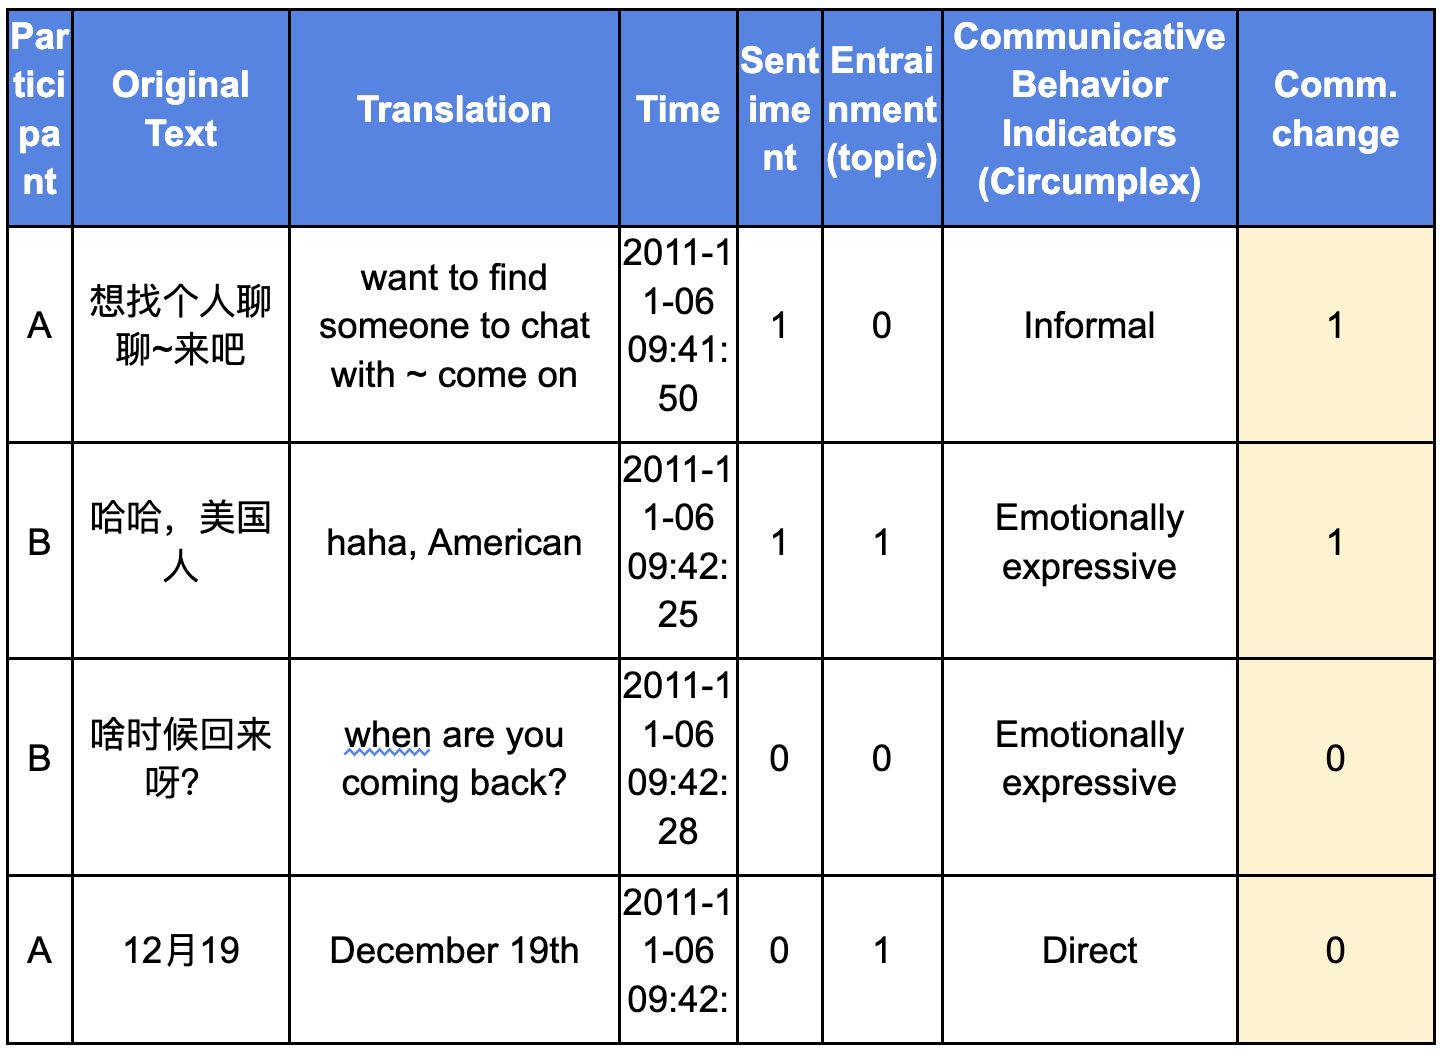
\includegraphics[width=0.75\textwidth]{sample_annotations.png}
    \caption{Sample annotations provided in the first change point labeling plan.}
    \label{fig:sample_annotations}
\end{figure}

One of Columbia's proposed approaches to the change point prediction task was to use circumplex theory as a proxy for the change point prediction task. Circumplex theory comes from the field of social psychology and aims to characterize interpersonal relations using a variety of social tags (see figure \ref{fig:circumplex}). The motivation for developing a circumplex theoretic system as a proxy for change point is as follows. If a circumplex theoretic system is easier to develop (e.g. because of existing data resources, etc.) and is highly correlated with the change point task, then we might improve the performance of our change point prediction system without the need for a large volume of change point prediction annotations.

\begin{figure}[H]
    \centering
    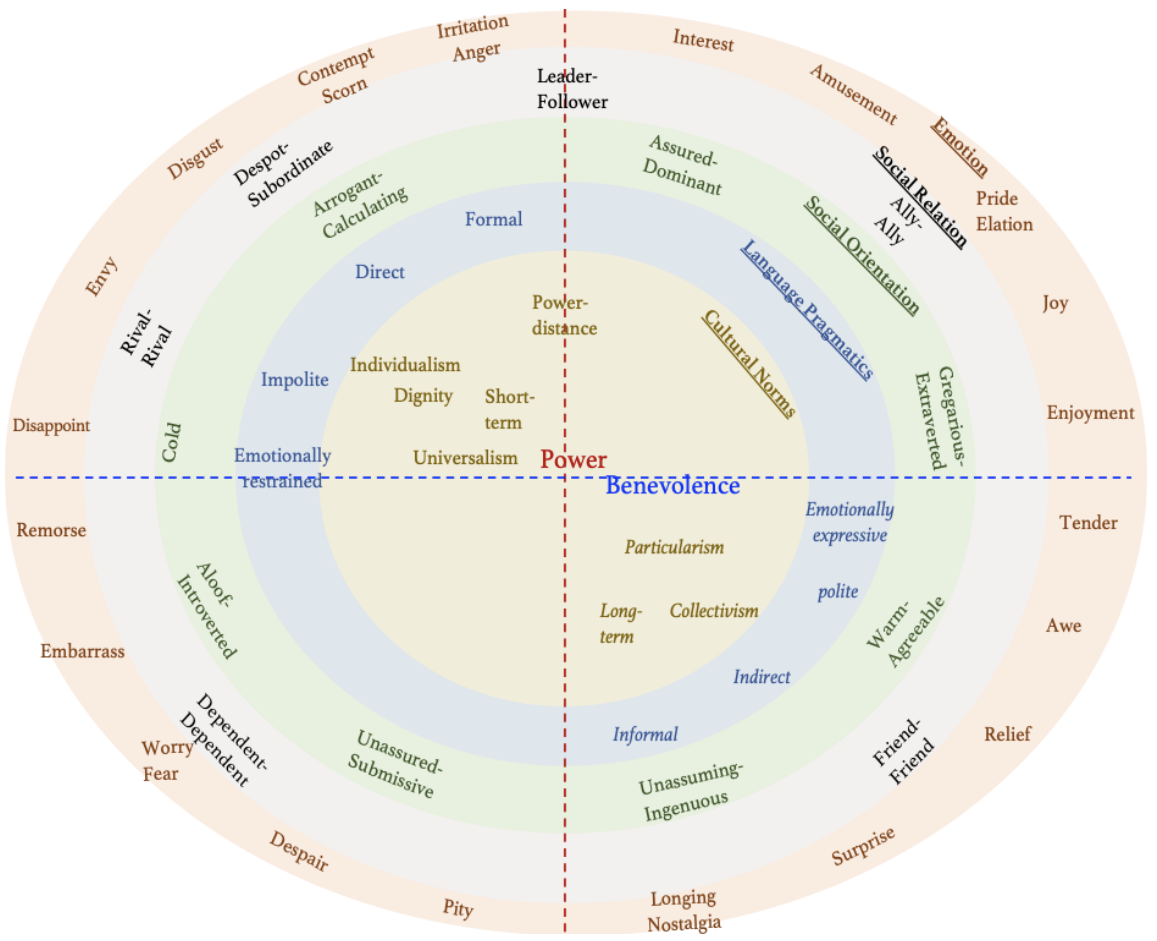
\includegraphics[width=0.75\textwidth]{circumplex.png}
    \caption{Circumplex diagram, where each concentric rings corresponds to tagging schemes to characterize interpersonal relations.}
    \label{fig:circumplex}
\end{figure}

In order to validate this approach, I developed a second data labeling plan focused on social relation tags \cite{Morrill_2022b}. Social relation tags characterize a person's behavior throughout an interaction and include the following tagset: \{Assured-Dominant, Gregarious-Extraverted, Warm-Agreeable, Unassuming-Ingenuous, Unassured-Submissive, Aloof-Introverted, Cold, Arrogant-Calculating\}. Yanda Chen and Yukun Huang volunteered to annotate several change point videos using the circumplex theory social relation tags. I then compared their predictions to the ground truth change point annotations provided by LDC and found that the social relation tagging scheme did correlate with change point prediction task. In particular, Yanda and Yukun's social relation tags found 100\% of the LDC change point annotations, though there were false positives (see figure \ref{fig:social_relation}). My sense is that social relation tags have the potential to be even more fine-grained than the change point task. These fine-grained predictions can then be fed to a downstream system that can filter through these social relation tags and decide what's useful for the change point prediction task.

\begin{figure}[H]
    \centering
    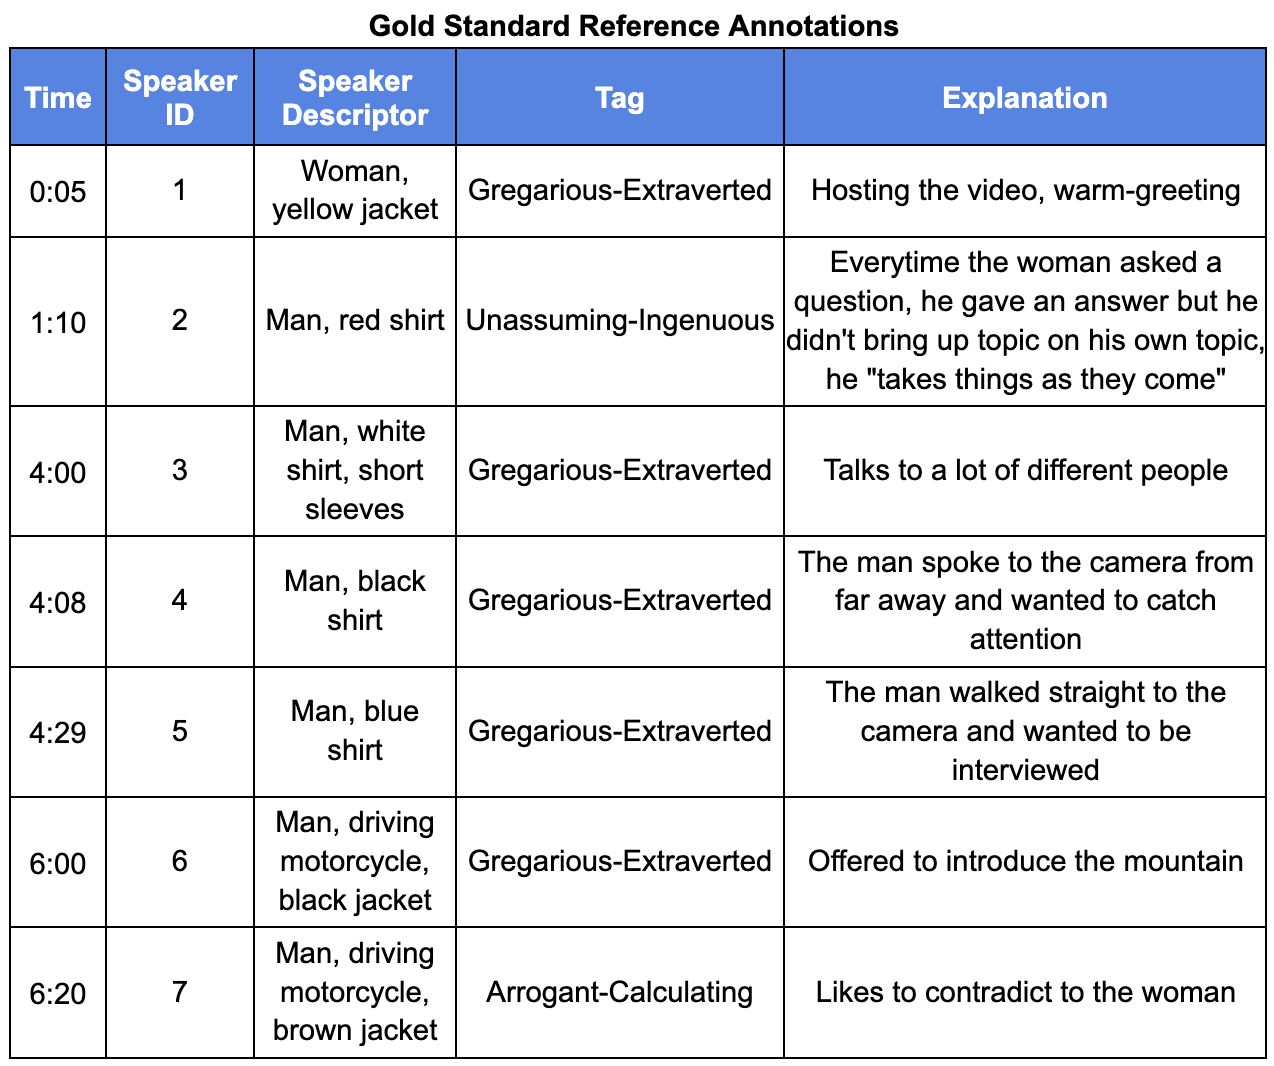
\includegraphics[width=0.75\textwidth]{social_relation_tags.png}
    \caption{Social relation tags for a \href{http://vd2.bdstatic.com/mda-ncqdcucf3m6zgjzz/360p/h264_delogo/1648202114325469972/mda-ncqdcucf3m6zgjzz.mp4}{sample video}.}
    \label{fig:social_relation}
\end{figure}

Throughout the semester, I met with and corresponded with Colin Leach, Professor of Psychology \& Africana Studies from Barnard College, who provided helpful guidance and resources. Professor Leach shared a dictionary of English words tagged to 128 categories such as positive emotion, negative emotion, affect, etc. (see figure \ref{fig:dictionary}). One approach to social relation tagging is weak supervision, whereby we tag each word in a person's utterance to a particular social relation tag. We can then create a signature of the person's social relation tag through summary statistics (e.g. sum the number of words used for each social relation tag).  

\begin{figure}[H]
    \centering
    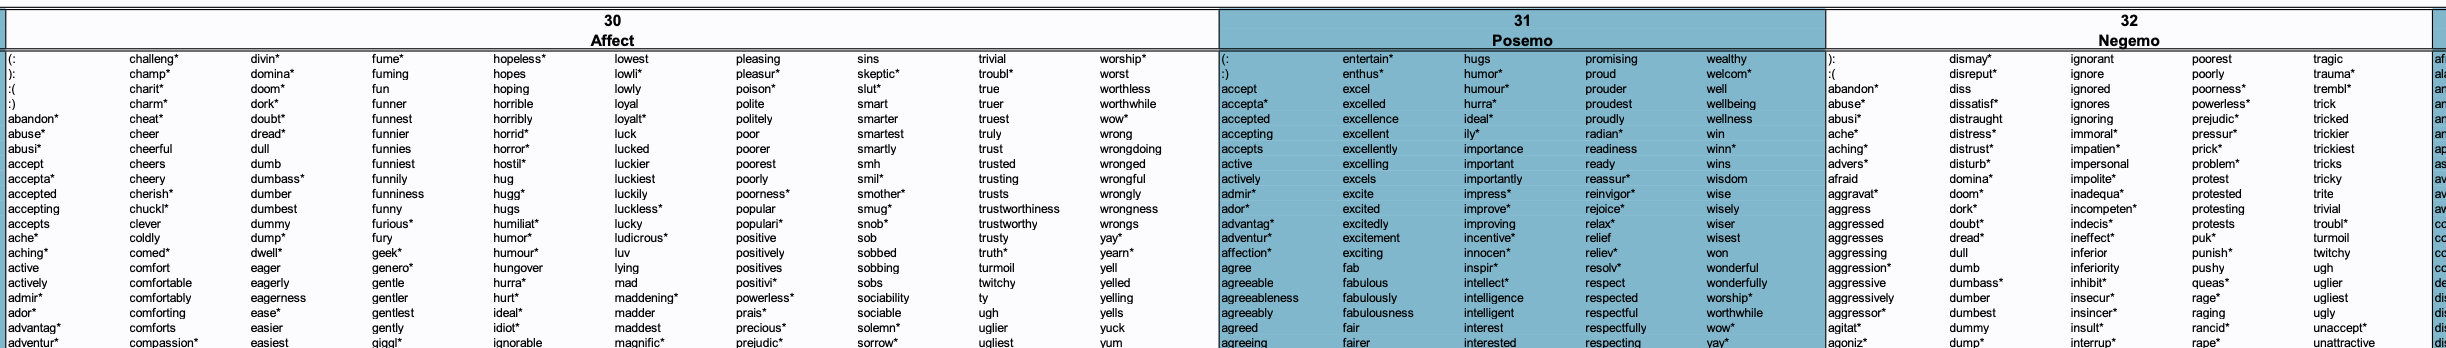
\includegraphics[width=1.0\textwidth]{dictionary.png}
    \caption{Dictionary of English words mapped to categories such as affect, positive emotion and negative emotions.}
    \label{fig:dictionary}
\end{figure}

\section{Integration}
Integration is the task of combining all of the systems developed for the DARPA CCU program across TA1 and TA2 teams. TA1 teams are responsible for social norm detection, emotion detection, and change point detection. TA2 teams are responsible for consuming the output of TA1 systems to inform operators (e.g. diplomats, military commanders, etc.) how their cross-cultural interactions are going and provide guidance to them so they can achieve their objectives. In addition to combining all the systems, the integration lead interfaces with LDC to inventory data releases and NIST to comply with the evaluation procedures of the program.

This semester I created a master inventory of all data releases along with useful metadata such as the modality, annotation status, etc. (see figure 
\ref{fig:metadata}). While creating this metadata inventory, I translated hundreds of LDC documents to English so that 1) English speakers could inspect the documents and 2) we could apply models trained on English data only. During this exercise, I accounted for all files that were transcribed and then worked with Sukrit Rao and Michael Picheny at New York University (NYU) to prioritize transcriptions for mini evaluation data. I shared this metadata artifact with the CHARM team internally at Columbia and it was immediately useful to those that used it (e.g. Tom Zollo). I also familiarized myself with Columbia's proposal for the DARPA CCU project, NIST's evaluation guidelines, and SRI's resources (e.g. Confluence, Docker containers, message queues, etc.). I attended weekly integration meetings and recently presented an overview of the change point systems developed for the mini evaluation so that TA2 teams have more insight into how to use our systems. Throughout the semester I have worked with Tom Zollo to raise questions and learn about the processes and code base that he has developed. 

\begin{figure}[H]
    \centering
    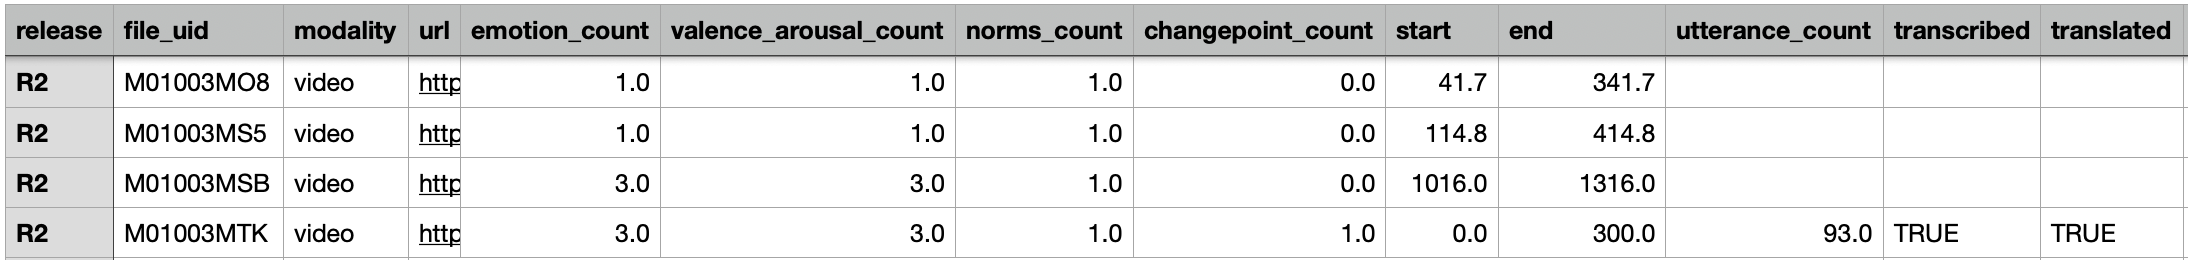
\includegraphics[width=1.0\textwidth]{metadata.png}
    \caption{Metadata sheet created to inventory all data releases.}
    \label{fig:metadata}
\end{figure}

\section{Next Steps}
\textbf{Change Point Data Annotation} Building on the social relation annotation scheme, I requested additional annotation support from Heng Ji, Professor of Computer Science at University of Illinois, Urbana-Champaign (UIUC), and her students. The goal is to train 2-4 students from UIUC to perform social relation annotations on approximately 100 videos that can be used as a test set. We will still require a training dataset to build models that can generate social relation tags. One approach to generating such a dataset is to prompt GPT-3 to annotate social relation tags for video transcriptions. A more precise approach, albeit more costly, is to use Amazon Mechanical Turk to annotate approximately 1,000 videos with social relation tags.

A parallel approach to producing social relation tags for social interactions is to come up with a mapping from the 128 dictionary categories to social relation tags. We can work with Professor Leach to derive a suitable mapping or pursue other lexicon resources.

\textbf{Integration} A primary goal for the integration workstream is to continue building a data loader that can be used by all CHARM team members. The LDC data releases contain terabytes of data, rendering it infeasible for individuals to download all of this data and manage it on their local laptops or desktops. A more scalable approach is to host this data on a central server, such as Google Drive, and build a Python library that can download files, as needed. Note that the metadata sheet generated this semester can help users subset the population of files that they would like to download.

Other integration goals include having TA1.* teams share system information with TA2 teams, sharing TA1.* system output with TA2 teams for development, using Git and Github for development, and easing the container development lifecycle so that we can test and ship working systems more regularly. Given the large responsibility of the integration role, we might consider seeking out another person to assist in achieving the goals listed above.
\printbibliography
\end{document}